% Chapter 1

\chapter{Software Implementation} % Write in your own chapter title
\label{Chapter2}
\lhead{Chapter 2. \emph{Software Implementation}} % Write in your own chapter title to set the page header
\section{Block Diagram}
\begin{tikzpicture}[]
	\node  (in1) [above=1cm,io, label={[yshift=-0.5cm]left:Input-\\ three-\\phase}]{};
	\node  (in2) [below=1cm of in1, io]{};
	\node (out1) [right= 13cm of in1]{};
	\node (out2) [right= 13cm of in2]{};
	\draw (in1)--node[pos=0.8,above=2pt]{$I_{out}$}(out1);
	\draw (in2)--(out2);
	\path (in1)--node[pos=0.5](a){}(in2)
	node[block,right=1cm of a](t){Rect-\\tifier}
	node[block,right=1cm of t](r){Filter}
	node[block,right=1cm of r](f){Inverter} 
	node[block,right=1cm of f](re){LCLfilter}
	node[block,right=1cm of re](l){Load}
	;
	\draw[->] (11,1.2)--+(0.5,0);
	\node[above right=0.2cm and 1cm] at (re){$+$};
	\node[right=1cm] at (re){$V_{out}$};
	\node[below right=0.2cm and 1cm] at (re){$-$};
	\pic at (2.5,2) [scale=0.2]{reti};
	\pic at (5.5,-2) [scale=0.2]{filted};
	\pic at (8,2) [scale=0.2]{mysine};
\end{tikzpicture}

\section{Rectifier}
Below is the Matlab Simulink Diagram of Controlled Rectifier
\begin{figure}[htbp]
	\centering
	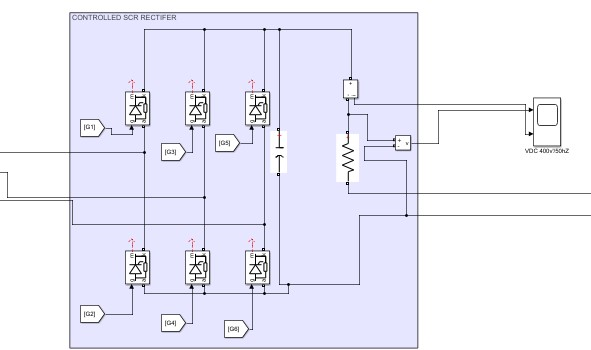
\includegraphics[width = 6in]{./Figures/rectifier1.jpg}
	\rule{35em}{1pt}
	\caption{Controlled Rectifier Block}
\end{figure}
The Controlled gate pulse Simulink Diagram
\begin{figure}[htbp]
	\centering
	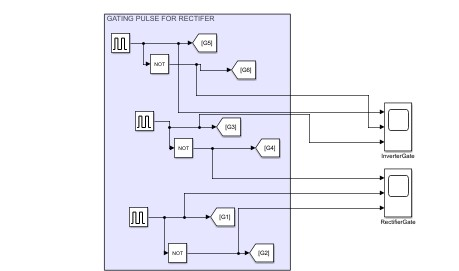
\includegraphics[width = 6in]{./Figures/rectifier2.jpg}
	\rule{35em}{1pt}
	\caption{Controlled Pulse Block}
\end{figure}
\newpage
\section{Inverter}
\subsection{SPWM Inverter}
\begin{figure}[htbp]
	\centering
	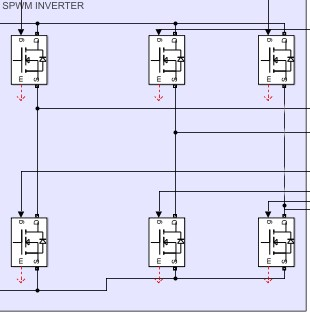
\includegraphics[width = 6in]{./Figures/Inverter.jpg}
	\rule{35em}{1pt}
	\caption{Inverter Block}
\end{figure}

\begin{figure}[htbp]
	\centering
	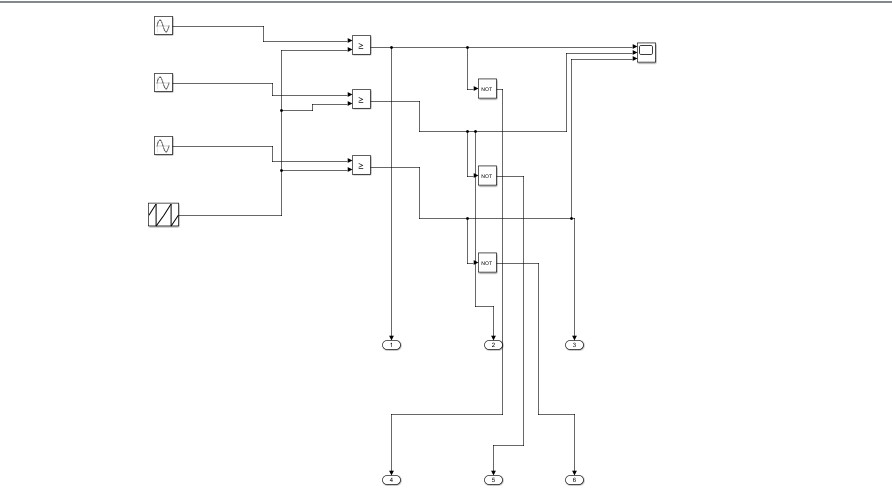
\includegraphics[width = 6in]{./Figures/Inverter1.jpg}
	\rule{35em}{1pt}
	\caption{Controlled Pulse Block}
\end{figure}
\newpage
\subsection{180 consuction Inverter}
\begin{figure}[htbp]
	\centering
	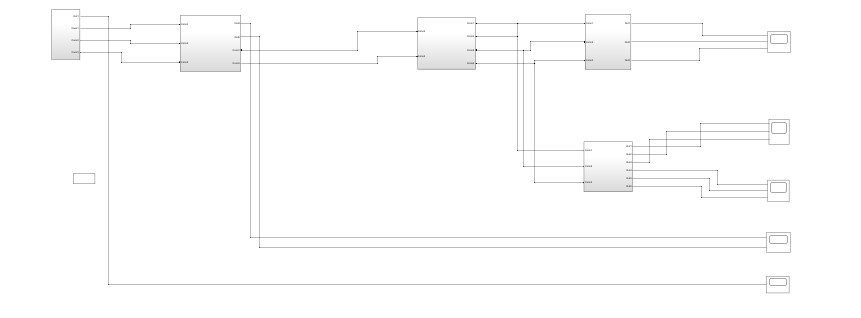
\includegraphics[width = 6in]{./Figures/180inverter.jpg}
	\rule{35em}{1pt}
	\caption{Simulink Diagram}
\end{figure}
\begin{figure}[htbp]
	\centering
	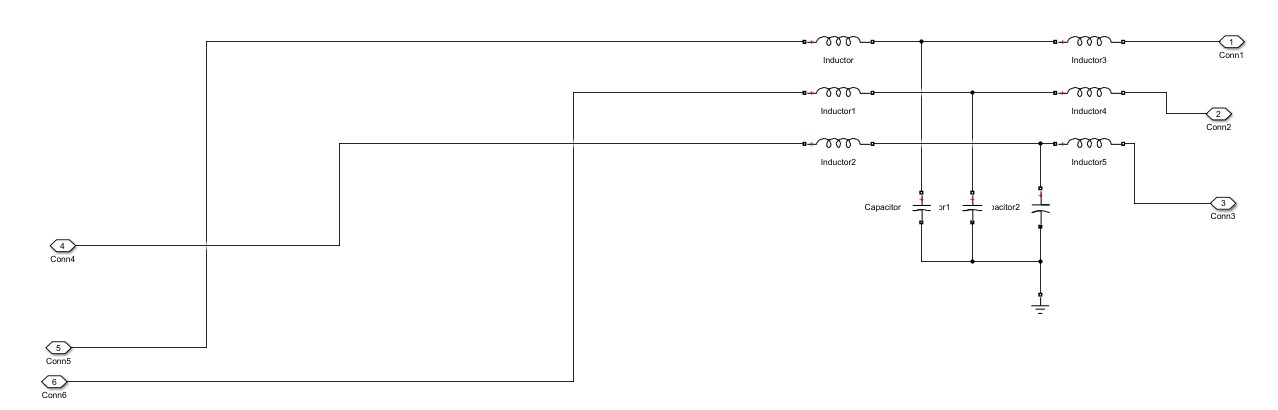
\includegraphics[width = 6in]{./Figures/LCL.jpg}
	\rule{35em}{1pt}
	\caption{LCL filter}
\end{figure}